\documentclass[a4paper,10pt]{book}

\usepackage[italian]{babel}
\usepackage{graphicx}
\usepackage[margin=2cm]{geometry}
\usepackage[utf8]{inputenc}
\usepackage{times}
\usepackage{float}
\usepackage{subfigure}
%\usepackage[left=2cm,right=1cm]{geometry}

%opening
\title{\begin{Huge}Multiple Description Streaming Protocol\end{Huge}\\Manuale Utente}
\author{}

\newcommand{\guikeys}[1]{\textit{#1}}
\newenvironment{notabene}{\begin{quote}\textbf{Nota bene.}}{\end{quote}}
\newenvironment{code}{\begin{quote}\vspace{0.5cm}\tt}{\vspace*{0.5cm}\end{quote}}   % Per i frammenti di codice.

\begin{document}
\frontmatter
\maketitle

\begin{figure}[b]
\vspace*{150pt}
{\small Eonio 2007,2008}
\vspace*{13pt}

{\small Scritto da Giuseppe D'Aqu\`i, Livio Pipitone}
\vspace*{13pt}

%{\small Editing a cura di Giuseppe D'Aqu\`i}
%\vspace*{13pt}

{\small Copertina di Andrea Delfino}
\vspace*{13pt}

{\footnotesize Ultimo aggiornamento: \today}
\vspace*{13pt}

\subfigure{
\includegraphics[width=1.5cm]{../images/cc.png}}

{\small Quest'opera \`e stata rilasciata sotto la licenza Creative Commons \textit{Attribuzione-Non commerciale-Condividi allo stesso modo 2.5 Italia}. Per leggere una copia della
licenza visita il sito web http://creativecommons.org/licenses/by-nc-sa/2.5/it/ o spedisci una lettera a Creative Commons, 171 Second Street, Suite 300, San Francisco, California, 94105, USA.}
\end{figure}

\tableofcontents



\chapter{Scopo}


\begin{itemize}
\item piattaforma per il test del protocollo mdc

\item progettazione e implementazione dei vari codec in un formato mdc-compatibile
\end{itemize}




\chapter{Codec}



\section{Definizione}


Un codec è un dispositivo (hardware o software) in grado di codificare e decodificare alcune informazioni in un formato di rappresentazione particolare. In genere il termine è usato in relazione a flussi multimediali (audio/video) processati tramite un elaboratore elettronico.






\section{Tipologie di codifica}


Le codifiche possono essere catalogate in differenti tipologie, ad esempio la tipologia 'Layered' ('a strati'), comune a tutti i codec MPEG.



Il Multiple Description Coding prevede che:
\begin{enumerate}
\item il flusso informativo sia suddiviso in più frammenti, detti 'Descrittori', con circa la stessa quantità di informazioni
\item i descrittori costituiscano due o più sotto-flussi;
\item i descrittori di un solo sotto-flusso, qualunque sia, devono bastare a ricostruire l'informazione, per lo meno con una bassa qualità
\item se vengono ricevuti due o più sotto-flussi, la qualità dell'informazione decodificata aumenta 
\end{enumerate}





\section{Differenze tra MDC e Layered}


La principale differenza tra la tipologia di codifica 'a descrittori multipli' e quella 'a strati' sta nella differente organizzazione delle informazioni: i frammenti ottenuti con una codifica MDC hanno potenzialmente lo stesso contenuto informativo in termini di quantità, mentre nei codec 'layered' esiste un frammento 'base', più importante degli altri, e diversi frammenti più piccoli di 'avanzamento'.






\chapter{Testbed}



\section{Organizzazione}


Il testbed è composto da un insieme di classi, suddivise in directory:



\begin{itemize}
\item 'common': classi che facilitano la realizzazione delle proprie applicazioni; comprendono utility per accedere alla rete, per simulare un comportamento multi-tasking, e altro.

\item 'codecs': contiene sia classi astratte, da usare come base per i codec reali, sia classi di utilità, come il registro dei codec, utilizzato per auto-caricare il codec adatto a seconda del flusso informativo

\item 'messages': l'iniseme dei messagi di base
\end{itemize}




\section{Implementazione}


Il testbed è stato sviluppato in C/C++, anche se, seguendo le specifiche, è possibile implementare una qualunque parte del sistema con qualsiasi linguaggio.






\section{Messaggi}


Le componenti del sistema che si trovano su elaboratori differenti comunicano tra loro per meggo di 'messaggi'. Tali messaggi rappresentano una particolare richiesta di servizi, oppure una corrispondente risposta.

Un messaggio possiede una 'tipologia' e un certo numero di 'argomenti', dipendenti dal tipo di messaggio.

Il tipico messaggio è composto da un header di 8 byte, cosi' suddivisi:



\begin{itemize}
\item 3 byte per la stringa MDC

\item 1 byte per la versione del protocollo

\item 4 byte per il tipo di messaggio
\end{itemize}

I messaggi possono avere un singolo parametro, oppure molti. Per 'parametro' qui ci si riferisce al parametro del messaggio, ovvero una stringa null-terminated, che a sua volta può contenere uno o più parametri a livello applicativo.






\subsection{LIST}
%

LIST



Composizione:



\begin{itemize}
\item header MDC

\item null-terminated string
\end{itemize}

la stringa può contenere una espressione regolare per la definizione del nome del flusso ricercato






\subsection{ALST}
%

Answer LiST



Lista di parametri






\subsection{SREQ}
%

Stream REQuest



Singolo parametro



\begin{itemize}
\item hash dello stream
\end{itemize}




\subsection{ASRQ}
%

Answer Stream ReQuest



Singolo parametro






\subsection{SINF}
%

Stream INFormation



Singolo parametro






\subsection{ASNF}
%

Answer Stream iNFormation



Singolo parametro






\subsection{PARM}
%

PARaMeters






\subsection{KALV}
%

Keep ALiVe



Singolo parametro






\subsection{PEER}
%

PEER



Singolo parametro






\subsection{APER}
%

Answer PEeR



Lista di parametri






\section{Descrittore}


Un 'Descriptor' è, nell'ambito di questo sistema, una unità di dati di un flusso multimediale.



Il flusso multimediale è suddiviso in sotto-flussi detti 'descrizioni', secondo le specifiche della codifica md; ogni descrizione è composta da un certo numero di descrittori, con la stessa relazione che c'è tra un filmato e un fotogramma.



Il Descriptor contiene varie informazioni, come il flusso originario, il numero di descrizione, e la sequenza temporale. Il payload non è definito e pertanto è permessa una maggiore libertà in fase di definizione dei codec.






\section{Casi d'uso}


Chiameremo Alice un generico nodo della rete che vuole effettuare le azioni, e Bob il peer a cui queste comunicazioni sono dirette.



Ci sono poi anche altri amici, come Carlina, David ed Emy, che condividono le stesse passioni di Alice e Bob.






\subsection{Richiesta di un flusso multimediale}
%

Alice ha bisogno di un flusso multimediale, e sa già che Bob ce l'ha, tutto o in parte (lo sa perché ha già visto la lista dei flussi di Bob).



Quindi Alice invia un messaggio SREQ, specificando come parametro l'hash univoco del flusso, il numero della descrizione, e una sequenza di descrittori.



Bob quindi invierà un messaggio ASRQ, specificando come parametro il timeout di keep-alive; Bob, infatti, continuerà ad inviare il flusso di dati finché riceverà pacchetti di KALV (keep-alive) da Alice, supponendola disconnessa allo scadere del timeout. 






\subsection{Richiesta della lista dei flussi}
%

\begin{itemize}
\item Alice ha bisogno della lista dei flussi disponibili da Bob. Invia un messaggio LIST, non parametro vuoto, e riceve da Bob un messaggio ALST (Answer LiST) contenente un vettore con tutti i nomi e gli hash dei flussi che egli possiede;

\item Alice sta cercando un particolare flusso, di cui sa parte del nome ('pippo'); invia un messaggio LIST a Bob con parametro '*pippo*', e Bob risponderà con un ALST contenente informazioni su tutti i file che contengono la parola 'pippo' nel nome.
\end{itemize}




\subsection{Richiesta di informazioni su un flusso}
%

Alice sa che un determinato flusso (di cui possiede l'hash) è posseduto da Bob; invia quindi un messaggio SINF (Stream INFormation), per avere informazioni specifiche del flusso, ad esempio la durata, la qualità di codifica, ecc. Bob invia un messaggio ASNF contenente la risposta.






\subsection{Invio di parametri di rete}
%

Alice deve informare Bob di cambiamenti che stanno avvenendo dalla sua parte; per esempio, sta cambiando rete e non vuole interrompere lo streaming; oppure c'è stato un problema con il router ed è necessario abbassare la velocità di invio del flusso. In tutti questi casi, Alice invia un messaggio PARM a Bob, specificando i nuovi parametri.






\subsection{Richiesta di altri peer con lo stesso flusso}
%

Alice sta scaricando un flusso da Bob, ma avverte la necessità di frequentare altre persone, che magari condividono lo stesso flusso; invia quindi un messaggio PEER a Bob, seguito dall'hash univoco del flusso. Bob raccoglie le idee su tutti gli amici che conosce, o che ha conosciuto tramite lo scaricamento del flusso in oggetto, per esempio Carlina, da cui Bob ha scaricato originariamente il flusso, David, che ha scaricato il flusso tempo fa, ed Emy che lo sta scaricando ora. Bob quindi prepara un messaggio APER contenente l'indirizzo ip e la porta di Carlina, David ed Emy e lo invia ad Alice.






\section{MDSP}


MDSP sta per Multiple Description Stream Protocol, ed è un protocollo per lo scambio di stream di vario tipo (contenuti multimediali) organizzati secondo una meta-codifica a descrittori multipli.






\mainmatter
\chapter{Analisi dei Requisiti}

\section{Modello \emph{Layered}}

\section{Modello \emph{Multiple Descriptions}}

\section{Scopo}


\begin{itemize}
\item piattaforma per il test del protocollo mdc

\item progettazione e implementazione dei vari codec in un formato mdc-compatibile
\end{itemize}




\section{Codec}



\section{Definizione}


Un codec è un dispositivo (hardware o software) in grado di codificare e decodificare alcune informazioni in un formato di rappresentazione particolare. In genere il termine è usato in relazione a flussi multimediali (audio/video) processati tramite un elaboratore elettronico.






\section{Tipologie di codifica}


Le codifiche possono essere catalogate in differenti tipologie, ad esempio la tipologia 'Layered' ('a strati'), comune a tutti i codec MPEG.



Il Multiple Description Coding prevede che:
\begin{enumerate}
\item il flusso informativo sia suddiviso in più frammenti, detti 'Descrittori', con circa la stessa quantità di informazioni
\item i descrittori costituiscano due o più sotto-flussi;
\item i descrittori di un solo sotto-flusso, qualunque sia, devono bastare a ricostruire l'informazione, per lo meno con una bassa qualità
\item se vengono ricevuti due o più sotto-flussi, la qualità dell'informazione decodificata aumenta 
\end{enumerate}





\section{Differenze tra MDC e Layered}


La principale differenza tra la tipologia di codifica 'a descrittori multipli' e quella 'a strati' sta nella differente organizzazione delle informazioni: i frammenti ottenuti con una codifica MDC hanno potenzialmente lo stesso contenuto informativo in termini di quantità, mentre nei codec 'layered' esiste un frammento 'base', più importante degli altri, e diversi frammenti più piccoli di 'avanzamento'.






\section{Testbed}



\section{Organizzazione}


Il testbed è composto da un insieme di classi, suddivise in directory:



\begin{itemize}
\item 'common': classi che facilitano la realizzazione delle proprie applicazioni; comprendono utility per accedere alla rete, per simulare un comportamento multi-tasking, e altro.

\item 'codecs': contiene sia classi astratte, da usare come base per i codec reali, sia classi di utilità, come il registro dei codec, utilizzato per auto-caricare il codec adatto a seconda del flusso informativo

\item 'messages': l'iniseme dei messagi di base
\end{itemize}




\section{Implementazione}


Il testbed è stato sviluppato in C/C++, anche se, seguendo le specifiche, è possibile implementare una qualunque parte del sistema con qualsiasi linguaggio.






\section{Messaggi}


Le componenti del sistema che si trovano su elaboratori differenti comunicano tra loro per meggo di 'messaggi'. Tali messaggi rappresentano una particolare richiesta di servizi, oppure una corrispondente risposta.

Un messaggio possiede una 'tipologia' e un certo numero di 'argomenti', dipendenti dal tipo di messaggio.

Il tipico messaggio è composto da un header di 8 byte, cosi' suddivisi:



\begin{itemize}
\item 3 byte per la stringa MDC

\item 1 byte per la versione del protocollo

\item 4 byte per il tipo di messaggio
\end{itemize}

I messaggi possono avere un singolo parametro, oppure molti. Per 'parametro' qui ci si riferisce al parametro del messaggio, ovvero una stringa null-terminated, che a sua volta può contenere uno o più parametri a livello applicativo.






\subsection{LIST}
%

LIST



Composizione:



\begin{itemize}
\item header MDC

\item null-terminated string
\end{itemize}

la stringa può contenere una espressione regolare per la definizione del nome del flusso ricercato






\subsection{ALST}
%

Answer LiST



Lista di parametri






\subsection{SREQ}
%

Stream REQuest



Singolo parametro



\begin{itemize}
\item hash dello stream
\end{itemize}




\subsection{ASRQ}
%

Answer Stream ReQuest



Singolo parametro






\subsection{SINF}
%

Stream INFormation



Singolo parametro






\subsection{ASNF}
%

Answer Stream iNFormation



Singolo parametro






\subsection{PARM}
%

PARaMeters






\subsection{KALV}
%

Keep ALiVe



Singolo parametro






\subsection{PEER}
%

PEER



Singolo parametro






\subsection{APER}
%

Answer PEeR



Lista di parametri






\section{Descrittore}


Un 'Descriptor' è, nell'ambito di questo sistema, una unità di dati di un flusso multimediale.

Il flusso multimediale è suddiviso in sotto-flussi detti 'descrizioni', secondo le specifiche della codifica md; ogni descrizione è composta da un certo numero di descrittori, con la stessa relazione che c'è tra un filmato e un fotogramma.

Il Descriptor contiene varie informazioni, come il flusso originario, il numero di descrizione, e la sequenza temporale. Il payload non è definito e pertanto è permessa una maggiore libertà in fase di definizione dei codec.






\section{Casi d'uso}


Chiameremo Alice un generico nodo della rete che vuole effettuare le azioni, e Bob il peer a cui queste comunicazioni sono dirette.

Ci sono poi anche altri amici, come Carlina, David ed Emy, che condividono le stesse passioni di Alice e Bob.


\subsection{Richiesta di un flusso multimediale}
%

Alice ha bisogno di un flusso multimediale, e sa già che Bob ce l'ha, tutto o in parte (lo sa perché ha già visto la lista dei flussi di Bob).



Quindi Alice invia un messaggio SREQ, specificando come parametro l'hash univoco del flusso, il numero della descrizione, e una sequenza di descrittori.



Bob quindi invierà un messaggio ASRQ, specificando come parametro il timeout di keep-alive; Bob, infatti, continuerà ad inviare il flusso di dati finché riceverà pacchetti di KALV (keep-alive) da Alice, supponendola disconnessa allo scadere del timeout. 






\subsection{Richiesta della lista dei flussi}
%

\begin{itemize}
\item Alice ha bisogno della lista dei flussi disponibili da Bob. Invia un messaggio LIST, non parametro vuoto, e riceve da Bob un messaggio ALST (Answer LiST) contenente un vettore con tutti i nomi e gli hash dei flussi che egli possiede;

\item Alice sta cercando un particolare flusso, di cui sa parte del nome ('pippo'); invia un messaggio LIST a Bob con parametro '*pippo*', e Bob risponderà con un ALST contenente informazioni su tutti i file che contengono la parola 'pippo' nel nome.
\end{itemize}




\subsection{Richiesta di informazioni su un flusso}
%

Alice sa che un determinato flusso (di cui possiede l'hash) è posseduto da Bob; invia quindi un messaggio SINF (Stream INFormation), per avere informazioni specifiche del flusso, ad esempio la durata, la qualità di codifica, ecc. Bob invia un messaggio ASNF contenente la risposta.






\subsection{Invio di parametri di rete}
%

Alice deve informare Bob di cambiamenti che stanno avvenendo dalla sua parte; per esempio, sta cambiando rete e non vuole interrompere lo streaming; oppure c'è stato un problema con il router ed è necessario abbassare la velocità di invio del flusso. In tutti questi casi, Alice invia un messaggio PARM a Bob, specificando i nuovi parametri.






\subsection{Richiesta di altri peer con lo stesso flusso}
%

Alice sta scaricando un flusso da Bob, ma avverte la necessità di frequentare altre persone, che magari condividono lo stesso flusso; invia quindi un messaggio PEER a Bob, seguito dall'hash univoco del flusso. Bob raccoglie le idee su tutti gli amici che conosce, o che ha conosciuto tramite lo scaricamento del flusso in oggetto, per esempio Carlina, da cui Bob ha scaricato originariamente il flusso, David, che ha scaricato il flusso tempo fa, ed Emy che lo sta scaricando ora. Bob quindi prepara un messaggio APER contenente l'indirizzo ip e la porta di Carlina, David ed Emy e lo invia ad Alice.






\section{MDSP}


MDSP sta per Multiple Description Stream Protocol, ed è un protocollo per lo scambio di stream di vario tipo (contenuti multimediali) organizzati secondo una meta-codifica a descrittori multipli.






\chapter{Progettazione}

\chapter{Implementazione}
\section{Codec}
\subsection{Codec testuale}
\label{cap:implementazione_codec}
Nel presente capitolo verrà descritto il funzionamento e l'implementazione
del codec testuale. L'analisi inizia da alcune considerazioni preliminari sul
file sorgente riguardanti la suddivisione delle informazioni secondo le
caratteristiche tipiche delle tecniche a descrizione multipla. Nella
implementazione di MDSP un file sorgente può essere suddiviso in uno o più
descrizioni, fino a un massimo di 64. Ogni descrizione, considerata
singolarmente, è in grado di descrivere l'intero file. \`E cioé sufficiente
alla corretta decodifica del file sorgente. Qualora il file sorgente venga
codificato in più di una descrizione sarà possibile la ricostruzione
perfetta del file esclusivamente nel caso in cui tutti le descrizioni giungano
a destinazione. Durante la procedura di decodifica del testo, MDSP versione 0.1
sostituisce un carattere \emph{spazio} qualora una lettera non giunga a
destinazione. Nel caso della decodifica di immagini viene sostituito il
pixel non giunto a destinazione con uno apportunamente scelto e
poi interpolato. Oltre tali accorgimenti, è necessario prendere in
considerazione l'eventualità che giunga a destinazione una singola descrizione
con alcuni descrittori errati (caso peggiore). Tale eventualità si risolve
facendo sì che durante la codifica i descrittori, ma ancor più le descrizioni,
contengano dati provenienti 'da tutte le zone del file'. Al fine del
raggiungimento di tale scopo, vengono di seguito riportati gli indici necessari
e alcune semplici formule per poterli colcolare:
\begin{itemize}
 \item Dimensione di ogni descrizione: $$\frac{dimensione\_file}{numero\_descrizioni}$$
 \item Numero di descrittori per ogni descrizione: $$\frac{dimensione\_descrizione}{dimensione\_descrittore}$$
 \item Dimensione di ogni descrittore: $$\frac{dimensione\_descrizione}{numero\_descrittori}$$
\end{itemize}
Tali accorgimenti non sono da soli sufficienti per la realizzazione di un codec
pienamente compatibile MDC, ulteriori accorgimenti verranno illustrati con
maggiore dettaglio nel capitolo \ref{cap:codec_esempio}.
\\\\
La struttura delle classi C++ di gestione dei codec comprende classi astratte
che regolano lo scambio di dati tra i codec e il motore di streaming, nonché la
composizione delle strutture dati in memoria da utilizzare. Le classi a cui ci si riferisce sono contenute nella directory \textit{mdc/src/codecs/}. Di
seguito vengono elencate e brevemente descritte le classi astratte per la
gestione dei codec:
\begin{itemize}
 \item \textit{abstract\_codec\_parameter.h}: astrae i parametri del codec; per
 utilizzare tale classe è necessario specificare il comportamento di essa nelle
 funzioni \textit{serialize()} e \textit{deserialize()}.
 \item \textit{abstract\_md\_codec.h}: astrae il funzionamento del codec a
 descrizioni multiple; per utilizzare tale classe è necessario specificare il
 comportamento di essa nelle funzioni \textit{code()} e \textit{decode()}. In
 tali funzioni è contenuto il cuore del codec e pertanto necessitano un'analisi
 più dettagliata, si rimanda al capitolo \ref{cap:codec_esempio}.
 \item \textit{abstract\_stream.h}: astrae la gestione dei dati specifici per il
 tipo di file sorgente considerato; per utilizzare tale classe è necessario
 specificare il comportamento di essa nelle funzioni \textit{load\_from\_disk()}
 e \textit{save\_to\_disk()}.
\end{itemize}

Di seguito vengono brevemente illustrati gli stralci di due file
testuali, il primo è il file sorgente e viene codificato in 4 descrizioni,
mentre il secondo è il file decodificato. A titolo dimostrativo viene riportata
la porzione di testo in cui una descrizione su 4 è andata perduta durante il
trasferimento:

\begin{itemize}
  \item \emph{``Se mai si racconterà la mia storia, si dica che ho camminato
  coi Giganti. Gli uomini sorgono e cadono come grano invernale, ma questi nomi non periranno mai. Si dica che ho vissuto al tempo di Ettore, domatore di cavalli... Si dica... che ho vissuto al tempo di Achille...'' (Ulisse - Troy)}
  \item \emph{``Se mai si  acc nte à l  mi  st ria  si dic  ch  ho cam ina o c
  i G gan i.  li  omi i s rgo o e cad no  ome gra o i ver ale  ma que ti  omi  
  non per ran o m i.  i d ca  he  o v ssu o a  te po  i E tor , d mat re  i
  c val i..  Si dic ... che ho  iss to  l t mpo di  chi le. .''  Uli se   Tr y)}
\end{itemize}

Si può notare la presenza del carattere \emph{spazio} al posto delle lettere
appartenenti alla descrizione persa.

\subsection{Codec grafico}
Per la realizzazione di un codec grafico sono richieste le stesse proprietà del
codec testuale (compatibilità MDC). Il codec grafico si differenzia dal codec
testuale in alcuni punti che verranno di seguito analizzati:

\begin{itemize}
  \item Durante la procedura di decodifica delle immagini, per ogni pixel
  non giunto a destinazione, MDSP versione 0.1 sostituisce un '\emph{pixel
  fantasma}'. Il pixel di default ha componenti RGB = 0,255,0. Questa
  tipologia di pixel viene utilizzata al fine dell'esecuzione dell'algoritmo
  descritto nel prossimo punto. MDSP versione 0.1 non permette all'utente di
  modificare tale valore, ma ci si propone di realizzare un interfacciamento a tale opzione nelle prossime versioni.
  \item Immediatamente dopo la decodifica, MDSP 0.1 esegue un algoritmo di
  interpolazione dei \emph{pixel fantasma} al fine di approssimare al meglio i
  pixel originari a partire dai pixel reali più prossimi. Con tale affermazione
  si intente la procedura di approssimazione di un \emph{pixel fantasma} con i
  suoi vicini esclusivamente se i vicini sono pixel con valore RGB diverso da
  0,255,0. Se un vicino possiede il valore RGB di defaul (se cioé è anch'esso
  un \emph{pixel fantasma}) viene scartato e si passa all'analisi del vicino di
  secondo ordine. In tale evenienza l'algoritmo viene eseguito ricorsivamente.
  La funzione in questione è contenuta nel file
  \textit{mdc/src/codecs/image/image\_stream.cpp} con il nome
  \textit{interpolate\_pixels()}
  \item Il formato di trasmissione dei pixel segue il formato della maschera,
  quindi RGB in quest'ordine. Nella realizzazione di questo tipo di codec è
  necessario gestire anche l'endianless e far sì che l'MD stream venga
  trasferito in formato big-endian (compatibile con il funzionamento delle reti
  di telecomunicazioni).
\end{itemize}

Il codec grafico contenuto in MDSP versione 0.1 permette la manipolazione di
immagini che possiedono una maschera di colori esclusivamente a 24 bit e di
file in formato BMP non compresso. Eventuali versioni future di MDSP potrebbero
supportare immagini di formato diverso e con diverse profondità di colore.
\\\\
Di seguito vengono brevemente illustrate due immagini, l'immagine
\ref{fig:sorgente} è il file sorgente e viene codificato in 4 descrizioni,
mentre l'immagine \ref{fig:decodificata} è il file decodificato.

\begin{figure}[ht]
\centering 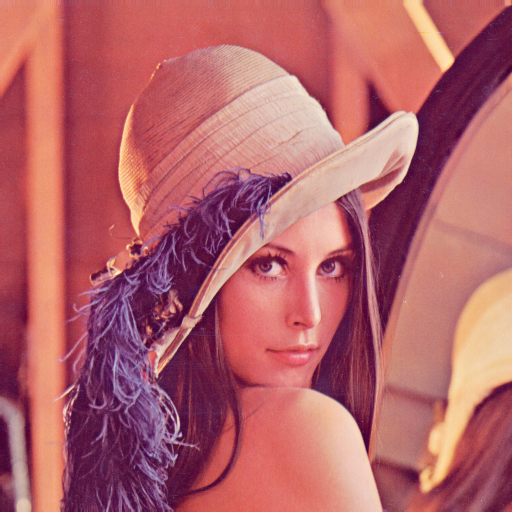
\includegraphics[width=0.90\textwidth]{../images/lena1.bmp}
	\caption{Immagine sorgente.}
	\label{fig:sorgente}
\end{figure}

\begin{figure}[ht]
\centering 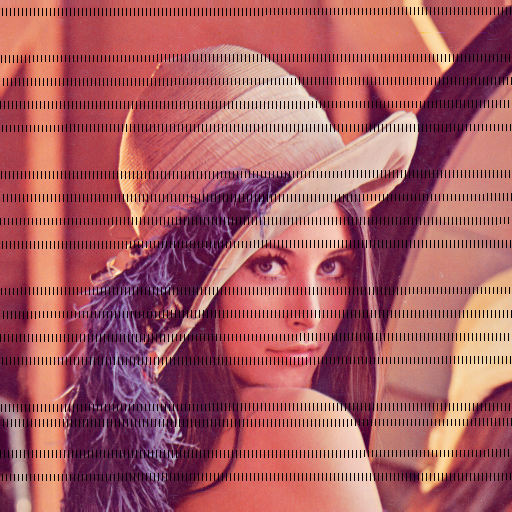
\includegraphics[width=0.90\textwidth]{../images/lena2.bmp}
	\caption{Immagine decodificata.}
	\label{fig:decodificata}
\end{figure}

Le immagini \ref{fig:sorgente} e \ref{fig:decodificata} permettono
l'immediata visione del funzionamento del codec nel suo complesso. Differentemente dal testo, l'immagine \ref{fig:sorgente} è stata
codificata e inviata al destinatario, successivamente è stata decodificata. La
perdita di descrittori (non descrizioni) è casuale e dovuta alla congestione o
inefficienza della rete. Tutte le descrizioni sono state correttamente
decodificate. Si può notare che l'immagine \ref{fig:decodificata} presenta delle
imperfezioni dovute esclusivamente alla perdita dei pixel associati ai descrittori persi
durante il trasferimento. In tali zone dell'immagine è stato eseguito
l'algoritmo di interpolazione.
\chapter{Manuale}
Nel presente capitolo verranno illustrati i principali comandi per la
transcodifica e la gestione del protocollo MDSP.

\section{Comandi principali}
I principali comandi riguardanti l'applicazione MDSP versione 0.1 sono relativi
alle operazioni di codifica, decodifica e avvio in modalità server e client. I
comandi relativi alla codifica e alla decodifica di seguito riportati sono
relativi all'uso di un file testuale. L'esempio è comunque valido nel caso si
vogliano utilizzare file contenenti immagini.

\begin{itemize}
  \item Codifica: \texttt{mdc --input text\_file.txt --code --codec text
  --output text\_file.mdc}\\ Per la codifica è strettamente necessario
  specificare il file sorgente (\emph{input}), il file di output, l'operazione desiderata (\emph{code}) e il
tipo di codec da utilizzare (\emph{text}). Nel paragrafo \ref{sec:opzioni} vengono riportate tutte le opzioni disponibili. 
  \item Decodifica: \texttt{mdc --input text\_file.mdc --decode --codec
  text\\ --output new\_text\_file.txt}\\ Per la decodifica è strettamente
  necessario specificare il file sorgente (\emph{input}), il file di output, l'operazione desiderata (\emph{decode}) e il
tipo di codec da utilizzare (\emph{text}). Nel paragrafo \ref{sec:opzioni} vengono riportate tutte le opzioni disponibili.
  \item Modalità server: \texttt{mdc --daemon}\\ Lanciando da linea di comando
  MDSP versione 0.1 in modalità server, l'applicazione viene configurata come `erogatore di file' e si pone in ascolto
sulle porte UDP 5551 per i segnali di controllo e 5552 per lo scambio dai dati. Nel capitolo \ref{cap:protocollo} viene illustrato nel dettaglio il
funzionamento e la configurazione della modalità di esecuzione server.
  \item Modalità client: \texttt{mdc}
\end{itemize}

\section{Opzioni}
\label{sec:opzioni}
Di seguito vengono elencate e descritte tutte le opzioni dell'applicazione:

\begin{itemize}
  \item \texttt{--input}: (\emph{parametro obbligatorio}) è il
  nome del file sorgente, il nome comprende anche l'eventuale path completo;
  \item \texttt{--output}: (\emph{parametro obbligatorio}) è il
  nome del file di destinazione (il file decodificato), il nome comprende anche l'eventuale path
  completo.
  \item \texttt{--code}: (\emph{parametro obbligatorio}) indica
  l'operazione da effettuare, in questo caso codifica del file sorgente nel suo equivalente
  \emph{`.mdc'}.
  \item \texttt{--input}: (\emph{parametro obbligatorio}) indica
  l'operazione da effettuare, in questo caso decodifica del file \emph{`.mdc'}
  nel formato del file di output.
  \item \texttt{--codec}: (\emph{parametro obbligatorio}) specifica il tipo di
  codec da utilizzare. MDSP versione 0.1 può utilizzare un codec testuale (\emph{text})
  e un codec grafico (\emph{image}).
  \item \texttt{--flows}: specifica il numero di descrizioni in cui verrà
  codificato il file corgente. Tale opzione è utilizzabile esclusivamente insieme all'opzione
  \texttt{--code}, altrimenti verrà ignorata. \`E possibile specificare un
  numero intero di descrizioni compreso tra 1 e 64, se tale opzione non viene
  specificata MDSP procederà alla codifica del file sorgente utilizzando 2
  descrizioni.
  \item \texttt{--payload}: specifica una preferenza sulla quantità di dati che
  si desidera vengano trasportati in ogni descrittore. MDSP può modificare tale
  valore allorquando l'utente specifichi un valore non compatibile con le
  specifiche. Tale opzione è utilizzabile esclusivamente insieme all'opzione
  \texttt{--code}, altrimenti verrà ignorata. Se si utilizza il codec testuale
  tale valore può essere impostato in un intervallo compreso tra 25 e 55000
  (l'unità di misura è il carattere). In caso venga utilizzato il codec grafico
  l'intervallo ammesso è compreso tra 10 e 18330 (l'unità di misura è il
  pixel). Se tale opzione non viene specificata MDSP procederà alla codifica
  del file sorgente impostando il parametro al valore 1000 indipendentemente dal codec utilizzato.
  \item \texttt{--daemon}: avvia MDSP in modalità server.
  \item \texttt{--help}: visualizza una breve descrizione delle modalità
  operative e dei parametri ammessi.\\
\end{itemize}

Esempi di utilizzo:

\begin{code}
mdc --input input\_file.bmp --codec image --code --flows 4 --payload
2000\\ --output output\_file.mdc\\\\
mdc --input input\_file.mdc --codec image --decode --output
new\_output\_file.bmp
\end{code}
\chapter{Esempio codec testuale}
\section{Codifica}
Qu\`i di seguito si procede alla descrizione dei principali comandi in linguaggio C++ che formano una funzione di codifica MDC compatibile.

\begin{notabene}
La dicitura \textit{flow} \`e viene usata con il significato di ``\emph{Descrizioni}''. Tale variazione rispetto alla nomenclatura presente in letteratura \`e stata adottata al fine di evitare la possibile confusione dovuta alla somiglianza dei termini ``\emph{Descrizioni}'' e ``\emph{Descrittori}''. In seguito, quindi, la parola ``\emph{Flussi}'' \`e da intendersi con il significato di ``\emph{Descrizioni}''.
\end{notabene}

\begin{itemize}
 \item \begin{code}
Uint32 flow\_dimension = (stream\_size/m\_flows\_number)+1;\\
Uint32 descriptors\_number = \\(Uint32)ceil(((double)flow\_dimension)/((double)m\_preferred\_payload\_size));\\
Uint16 max\_payload\_size = (flow\_dimension/descriptors\_number)+1;\\
\end{code}

Innanzitutto \`e necessario calcolare dimensione e numero di flussi e descrittori. Il numero di descrittori da generare viene calcolato tenendo conto della \emph{dimensione preferita}, impostata dall'utente tramite linea di comando con il parametro \emph{--payload}; viene altres\`i utilizzata la dimensione predefinita nel caso non venga impostato alcun parametro. Si tratta di un parametro \emph{preferito} poich\`e il codec ha l'obiettivo di generare \emph{N} flussi sui quali devono essere distribuiti in modo possibilmente eguale i dati del file sorgente. Il parametro \textit{max\_payload\_size} ha quindi il compito di bilanciare il carico tra i flussi.

 \item \begin{code}
md\_stream->init(stream->compute\_hash\_md5(), m\_flows\_number, descriptors\_number);\\
\end{code}
Si inizializza un oggetto di tipo \textit{md\_stream} (Multiple Description Stream) con un codice hash MD5 che viene calcolato a partire dal file sorgente su disco, si specificano altres\`i il numero di flussi e di descrittori.

 \item \begin{code}
Descriptor* descriptor = new Descriptor();\\
descriptor->set\_stream\_id(md\_stream->get\_stream\_id());\\
descriptor->set\_flow\_id(i);\\
descriptor->set\_sequence\_number(j);\\
descriptor->set\_codec\_name(string("text"));\\
\end{code}
L'n-esimo descrittore viene inizializzato in memoria e viene impostato il parametro \textit{stream\_id} copiandolo da quello generato dal file sorgente su disco. Successivamente viene inserito il numero di flusso e sequenza che lo contraddistingue tra tutti gli altri descrittori del file. Il numero di sequenza viene incrementato per ogni nuovo descrittore ed è unico all'interno di un flusso. Con esso si pu\`o distinguere un descrittore all'interno di un flusso, la coppia di parametri (\textit{flow\_id}, \textit{descriptor}) individua un descrittore e lo distingue da tutti gli altri nell'ambito dell'intero file. Infine viene impostato il nome del codec che contrassegna ogni descrittore. Tale nome ha lo scopo di identificare, in fase di decodifica, il tipo di dati contenuti all'interno di un descrittore.

 \item \begin{code}
TextCodecParameters* tcp = new TextCodecParameters();\\
descriptor->set\_codec\_parameter(tcp);\\
\end{code}
Viene inizializzato un oggetto \textit{tcp} di tipo TextCodecParameters che contiene i parametri del codec. Poich\`e il testo semplice non possiede parametri significativi, tale oggetto viene inizializzato vuoto. Dopo la creazione, viene anch'esso associato al descrittore.

 \item \begin{code}
MemDataChunk payload;\\
Uint64 k;\\
for (k=0; k<max\_payload\_size; k++)\\
	if (offset+i+k+m\_flows\_number < stream\_size)\\
		payload += \&stream->get\_data(offset+i+(k*m\_flows\_number), 1);\\
offset += m\_flows\_number*k;\\
descriptor->set\_payload(payload);\\
\end{code}
Terminata la fase di preparazione del descrittore, si passa alla fase del riempimento con i dati prelevati dal file sorgente su disco. Viene inizializzata in memoria una struttura dati che consente di caricare porzioni di file da disco. Con un ciclo for vengono prelevati i caratteri dal file sorgente e inseriti nella struttura dati creata. l parametro \textit{offset} e la formula che lo contiene consetono di rispettare i vincoli di codifica, si tratta dei vincoli illustrati nel capitolo \ref{cap:descrizione_codec}. Finita la preparazione del payload, quest'ultimo viene accodato al descrittore che adesso risulter\`a completo.

 \item \begin{code}
md\_stream->set\_descriptor(descriptor);\\
\end{code}
Infine, l'N-esimo descrittore viene accodato al Multiple Description Stream per poter successivamente essere inviato.
\end{itemize}
In appendice \`e riportato il codice completo della funzione di codifica testuale appena descritta.

\section{Decodifica:}


\begin{itemize}
 \item \begin{code}
Uint8 flows\_number = md\_stream->get\_flows\_number();\\
Uint32 sequences\_number = md\_stream->get\_sequences\_number();\\
\end{code}
Dopo aver controllato che il Multiple Description Stream non sia vuoto, si creano due variabili contenenti il numero di flussi e delle sequenze dello stream (si ricordi che rispettivamente indicano il numero di descrizioni dello stream e di descrittori di ogni descrizione).

 \item \begin{code}
payload\_size = descriptor->get\_payload\_size();\\
if (md\_stream->is\_valid(descriptor->get\_flow\_id(), descriptor->get\_sequence\_number()))\{
	(*dc) += (descriptor->get\_payload());\\
	taken\_stream.resize(flows\_number*sequences\_number*(payload\_size+1));\\
	Uint8 current\_received\_data;\\
	Uint64 k;\\
	for (k=0; k<payload\_size; k++) \{\\
		dc->extract\_head(current\_received\_data);\\
		if (current\_received\_data != 0) \{\\
			Uint64 locate\_position = offset+i+(k*flows\_number);\\
			taken\_stream[locate\_position] = current\_received\_data;\\
			if (locate\_position > max\_dimension)\\
			max\_dimension = locate\_position;\\
		\}\\
	\}\\
	offset += flows\_number*k;\\
\}\\
\end{code}
La porzione di codice che si sta per analizzare \`e di fondamentale importanza. Tutte le operazioni vengono effettuate sul descrittore correntemente selezionato, quindi si eviter\`a di ripeterlo. Innanzitutto viene memorizzata la dimensione del payload, tale dimensione \`e costante e pu\`o variare esclusivamente per l'ultimo descrittore di un flusso.
\begin{notabene}
Non ha senso effettuare paragoni tra descrittori appartenenti a flussi diversi, in quanto non sono in alcun modo correlati.
\end{notabene}
Se il descrittore corrente viene ritenuto valido all'interno del Multiple Description Stream si passa alla decodifica. Viene prelevato il payload e trasferito in una struttura dati in memoria (Memory DataChunk). Il contenitore temporaneo dello stream decodificato viene ridimensionato per contenere (potenzialmente) tutti i payload provenienti da tutti i descrittori. \`E possibile raggiungere la dimensione massima esclusivamente nel caso in cui non vi sia alcun errore di trasmissione. Successivamente si prelevano le singole lettere dalla struttura dati in memoria. Se la i-esima lettera estratta ha un codice ascii diverso da ``\emph{0}'' si passa al calcolo della sua posizione assoluta all'interno dello stream finale (decodificato) e al posizionamento del carattere corrente in tale posizione. Infine viene aggiornato un contatore che tiene conto della massima posizione raggiunta in tale fase. Tale contatore servir\`a successivamente, pertanto il suo significato verr\`a descritto in seguito.

 \item \begin{code}
else\{\\
	Uint64 k;\\
	for (k=0; k<payload\_size; k++) \{\\
		Uint64 locate\_position = offset+i+(k*flows\_number);\\
		taken\_stream[locate\_position] = ' ';\\
	\}\\
	offset += flows\_number*k;\\
\}\\
\end{code}
Nel caso in cui il descrittore corrente, per qualunque motivo, non sia valido vengono calcolate tutte le posizioni nello stream finale relative alle lettere contenute nel suo payload che sono considerate perse. Al loro posto vengono sostituiti dei caratteri ``\emph{spazio}''. Esclusa quest'ultima variazione, l'algoritmo rimane del tutto simile a quanto visto sin'ora.

 \item \begin{code}
MemDataChunk* taken\_dc = new MemDataChunk();\\
Uint8* temp\_container = new Uint8[max\_dimension+1];\\
for (Uint64 i=0; i<max\_dimension+1; i++)\\
	temp\_container[i] = taken\_stream[i];\\
taken\_dc->append\_data(max\_dimension+1, temp\_container);\\
\end{code}
Terminata l'analisi di tutti i descrittori validi si devono rendere comprensibili (oltre che validi) i dati ricevuti. Si crea una lista di puntatori a locazioni da 8 bit (quindi caratteri) di dimensione pari all'estensione della porzione di stream decodificata correttamente. Se tutti i descrittori analizzati si sono rivelati validi tale dimensione coincider\`a con quella dello stream inviato dalla sorgente. Se, invece, saranno presenti errori tale dimensione sar\`a minore di quella originale. La dimensione della porzione di stream valido \`e di fondamentale importanza poich\`e segner\`a il limite entro il quale ogni puntatore della lista ``punta'' ad un valore realmente utile della memoria e non ad un valore impredicibile. Si procede successivamente al travaso dei dati dallo stream temporaneo alla lista di puntatori. L'ultima istruzione inserisce nell'apposita struttura dati in memoria il contenuto della lista di puntatori.

 \item \begin{code}
stream->set\_data(*taken\_dc);\\
\end{code}
Il comando finale riempie lo stream con le lettere presenti nella struttura dati appena preparata.
\end{itemize}
In appendice \`e riportato il codice completo della funzione di codifica testuale appena descritta.
\appendix
\chapter{Appendice}
\section{Funzione di codifica testuale}

La funzione di codifica testuale \`e contenuta nel file \textit{text\_md\_codec.cpp} presente nella directory \textit{mdc/src/codecs/text/}.

\begin{code}
void TextMDCodec::code(AbstractStream* stream, MDStream* md\_stream) const \{\\
	Uint32 stream\_size = stream->get\_data\_dim();\\
	Uint32 flow\_dimension = (stream\_size/m\_flows\_number)+1;\\
	Uint32 descriptors\_number = \\(Uint32)ceil(((double)flow\_dimension)/((double)m\_preferred\_payload\_size));\\
	Uint16 max\_payload\_size = (flow\_dimension/descriptors\_number)+1;\\
	md\_stream->init(stream->compute\_hash\_md5(), m\_flows\_number, descriptors\_number);\\
	for (Uint8 i=0; i<m\_flows\_number; i++) \{\\
		Uint64 offset = 0;\\
		for (Uint32 j=0; j<descriptors\_number; j++) \{\\
			if (stream\_size-(offset+i) > 0) \{\\
				Descriptor* descriptor = new Descriptor();\\
				descriptor->set\_stream\_id(md\_stream->get\_stream\_id());\\
				descriptor->set\_flow\_id(i);\\
				descriptor->set\_sequence\_number(j);\\
				descriptor->set\_codec\_name(string("text"));\\
				TextCodecParameters* tcp = new TextCodecParameters();\\
				descriptor->set\_codec\_parameter(tcp);\\
				MemDataChunk payload;\\
				Uint64 k;\\
				for (k=0; k<max\_payload\_size; k++)\\
					if (offset+i+k+m\_flows\_number < stream\_size)\\
						payload += \&stream->get\_data(offset+i+(k*m\_flows\_number), 1);\\
				offset += m\_flows\_number*k;\\
				descriptor->set\_payload(payload);\\
				md\_stream->set\_descriptor(descriptor);\\
			\}\\
		\}\\
	\}\\
\}\\
\end{code}

\begin{notabene}
La dicitura \textit{flow} \`e viene usata con il significato di ``\emph{Descrizioni}''. Tale variazione rispetto alla nomenclatura presente in letteratura \`e stata adottata al fine di evitare la possibile confusione dovuta alla somiglianza dei termini ``\emph{Descrizioni}'' e ``\emph{Descrittori}''. In seguito, quindi, la parola ``\emph{Flussi}'' \`e da intendersi con il significato di ``\emph{Descrizioni}''.
\end{notabene}

\section{Funzione di decodifica testuale}

La funzione di decodifica testuale \`e contenuta nel file \textit{text\_md\_codec.cpp} presente nella directory \textit{mdc/src/codecs/text/}.

\begin{code}
void TextMDCodec::decode(const MDStream* md\_stream, AbstractStream* stream) const \{\\
	if (md\_stream->is\_empty()) \\
		return;\\
	LOG\_INFO("Decoding...");\\
	MemDataChunk* dc = new MemDataChunk();\\
	vector<Uint8> taken\_stream;\\
	Uint8 flows\_number = md\_stream->get\_flows\_number();\\
	LOG\_INFO("Flows number: "$<<$flows\_number);\\
	Uint32 sequences\_number = md\_stream->get\_sequences\_number();\\
	LOG\_INFO("Sequences number: "$<<$sequences\_number);\\
	Uint64 max\_dimension = 0;\\
	for (Uint8 i=0; i<flows\_number; i++)\{
		Uint64 offset = 0;\\
		Uint16 payload\_size = 0;\\
		for (Uint32 j=0; j<sequences\_number; j++)\{
			Descriptor* descriptor = new Descriptor();\\
			if(!(descriptor->get\_codec\_name()=="text"))\\
			continue;\\
			if (md\_stream->get\_descriptor(i, j, descriptor))\{
				payload\_size = descriptor->get\_payload\_size();\\
				if (md\_stream->is\_valid(descriptor->get\_flow\_id(), descriptor->get\_sequence\_number()))\{
					(*dc) += (descriptor->get\_payload());\\
					taken\_stream.resize(flows\_number*sequences\_number*(payload\_size+1));\\
					Uint8 current\_received\_data;\\
					Uint64 k;\\
					for (k=0; k<payload\_size; k++) \{\\
						dc->extract\_head(current\_received\_data);\\
						if (current\_received\_data != 0) \{\\
							Uint64 locate\_position = offset+i+(k*flows\_number);\\
							taken\_stream[locate\_position] = current\_received\_data;\\
							if (locate\_position > max\_dimension)\\
								max\_dimension = locate\_position;\\
						\}\\
					\}\\
					offset += flows\_number*k;\\
				\}\\
			\}\\
			else\{\\
				Uint64 k;\\
				for (k=0; k<payload\_size; k++) \{\\
					Uint64 locate\_position = offset+i+(k*flows\_number);\\
					taken\_stream[locate\_position] = ' ';\\
				\}\\
				offset += flows\_number*k;\\
			\}\\
		\}\\
	\}\\
	MemDataChunk* taken\_dc = new MemDataChunk();\\
	Uint8* temp\_container = new Uint8[max\_dimension+1];\\
	for (Uint64 i=0; i<max\_dimension+1; i++)\\
		temp\_container[i] = taken\_stream[i];\\
	taken\_dc->append\_data(max\_dimension+1, temp\_container);\\
	stream->set\_data(*taken\_dc);\\
\}\\
\end{code}

\begin{notabene}
La dicitura \textit{flow} \`e viene usata con il significato di ``\emph{Descrizioni}''. Tale variazione rispetto alla nomenclatura presente in letteratura \`e stata adottata al fine di evitare la possibile confusione dovuta alla somiglianza dei termini ``\emph{Descrizioni}'' e ``\emph{Descrittori}''. In seguito, quindi, la parola ``\emph{Flussi}'' \`e da intendersi con il significato di ``\emph{Descrizioni}''.
\end{notabene}

\end{document}